% IEEE conference format, A4. Compile: pdflatex main && bibtex main && pdflatex main && pdflatex main
\documentclass[conference,a4paper]{IEEEtran}
\usepackage[T1]{fontenc}
\usepackage{amsmath}
\usepackage{graphicx}
\usepackage{booktabs}
\usepackage{cite}
\usepackage{url}
\usepackage{microtype}
\usepackage[hidelinks]{hyperref}
\newcommand{\pmstd}[2]{#1\,$\pm$\,#2}
\graphicspath{{figures/}}

\begin{document}

\title{Beyond the Single Split: A Reproducible Benchmark of Bengali Book Review Sentiment Classification with Explanations and Label-Noise Analysis}

\author{\IEEEauthorblockN{Anonymous Authors}
\IEEEauthorblockA{Affiliation withheld for review}}

\maketitle

\begin{abstract}
Reported accuracies for Bengali book-review sentiment are hard to compare: they often come from a single split of a small corpus, against weak baselines, with labels derived from star ratings. We re-examine the problem with repeated stratified cross-validation on a 2,009-review corpus (BBR-2009) rebuilt from the Mendeley and BanglaBook sources. Recurrent models trained from scratch reach at most 81.1\% accuracy, and one model's accuracy swings by 13 points between folds, so a single split can tell very different stories. Frozen pretrained embeddings lift the same models to 87.6\%. Fine-tuned BanglaBERT reaches \pmstd{93.8}{1.1}\%, ahead of XLM-R (91.3\%), multilingual BERT (86.8\%) and a TF-IDF SVM (90.2\%), while a larger model and an ensemble add nothing statistically reliable. On the Mendeley corpus BanglaBERT reaches \pmstd{96.7}{1.2}\%, yet a plain TF-IDF Naive Bayes already reaches 94.2\%, far above the 84\% reported earlier on a larger corpus. SHAP explanations pass a deletion test. Of the model's errors, 62\% are confident disagreements concentrated in rating-derived labels (8.6\% of BanglaBook reviews against 1.3\% of Mendeley reviews), and a blind audit by one LLM annotator suggests that many are label errors. On the official BanglaBook benchmark we reach 0.927 weighted F1, 0.6 points below the published value, so we make no state-of-the-art claim.
\end{abstract}

\begin{IEEEkeywords}
Bengali sentiment analysis, book reviews, BanglaBERT, cross-validation, label noise, SHAP
\end{IEEEkeywords}

\section{Introduction}
Readers post opinions about Bengali books online in large numbers, and a good sentiment classifier could make that stream of reviews useful. The text is hard to work with: spelling varies, writing is informal, emoji are common, and labeled data is scarce.

There is also a quieter problem. Many results on Bengali book reviews come from a single split of a small corpus. With 400 test reviews, the 95\% confidence interval at 95\% accuracy is already about $\pm 2$ points, so ranking models on one split tells us little. Our own cross-validation shows how bad it can get: the best recurrent model scores anywhere between 72.6\% and 85.8\% depending on the fold, so the headline number depends a great deal on which reviews happen to be held out.

We therefore ask a plain question: \emph{what do the numbers look like when the evaluation is done carefully?} Our contributions are:
\begin{itemize}
\item A cross-validated benchmark of twelve recurrent models, nineteen classical classifiers and four pretrained transformers, with repeated seeds, significance tests and calibration (Sections~\ref{sec:setup} and~\ref{sec:results}).
\item Evidence that single-split figures are unstable (one model's fold accuracies span 13 points), that a simple TF-IDF Naive Bayes already reaches 94.2\% on the public Mendeley reviews, far above the 84\% reported earlier on a larger corpus, and that Bengali pretraining matters more than model size or recurrence.
\item A label-noise analysis: confident errors cluster in rating-derived labels, and a blind re-annotation audit suggests that many of them really are label errors.
\item A SHAP study with a deletion-based faithfulness check, and a frank comparison with the official BanglaBook and Rokomari results, where we claim no state of the art.
\end{itemize}
We also release the corpus construction, the fold assignments and a datasheet.

\section{Related Work}
Early sentiment classifiers paired Naive Bayes, logistic regression or SVMs with TF-IDF features \cite{pang2002}. Recurrent networks \cite{mikolov2010}, gated cells \cite{hochreiter1997,cho2014}, bidirectional reading \cite{schuster1997} and attention \cite{bahdanau2015,wang2016} became the standard next, until the Transformer \cite{vaswani2017} and BERT-style pretraining \cite{devlin2019} changed the field again. BanglaBERT \cite{bhattacharjee2022} is an ELECTRA model pretrained on a large Bengali corpus, and XLM-R \cite{conneau2020} is a multilingual alternative.

Work on Bengali includes multilingual BERT transfer by Islam \emph{et al.}\ \cite{islam2020}, a comparison of classical and neural models by Hasan \emph{et al.}\ \cite{hasan2020}, and transformer models by Bhowmick and Jana \cite{bhowmick2021}. For book reviews, Hossain \emph{et al.}\ reported 84\% with Naive Bayes on their own 2,000-review corpus \cite{hossain2020}; Sarker \emph{et al.}\ reached 88.95\% weighted F1 with XLM-R on Rokomari reviews \cite{sarker2022}; and BanglaBook \cite{kabir2023} offers 158,065 rating-labeled reviews, on which BanglaBERT-large scores about 0.93 weighted F1. To our knowledge, no earlier study combines repeated cross-validation with significance tests, quantifies the effect of rating-derived labels, or checks whether token attributions are faithful for Bengali book reviews.

\section{Data and Experimental Setup}\label{sec:setup}
\begin{figure*}[!t]
\centering
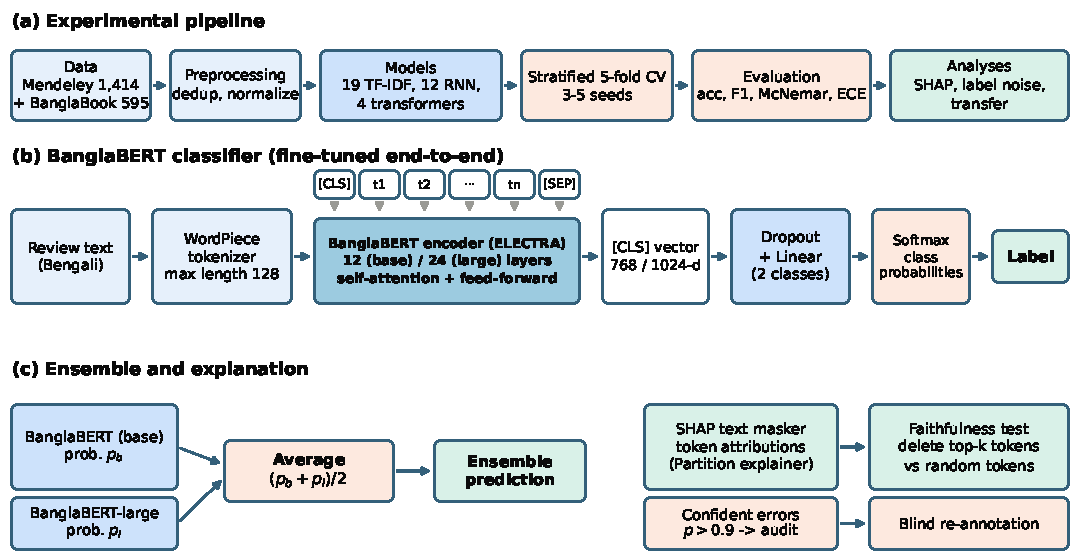
\includegraphics[width=\textwidth]{fig1_arch.pdf}
\caption{Overview. (a) Experimental pipeline. (b) The BanglaBERT classifier: the review is tokenized, encoded by the ELECTRA encoder, and the [CLS] vector feeds a dropout and linear layer. (c) Base and large probabilities are averaged, and token attributions and confident errors are analyzed afterwards.}
\label{fig:arch}
\end{figure*}
\subsection{Data}
\textbf{BBR-2009} contains 2,009 unique reviews (980 positive, 1,029 negative). We built it from 1,414 reviews of the Mendeley Bengali Book Reviews corpus (manually labeled, CC BY 4.0) and 595 reviews from BanglaBook \cite{kabir2023} (562 negative, 33 positive; star ratings 1--2 mapped to negative and 5 to positive; CC BY-NC-SA 4.0). It is a reconstruction from these public sources. Because the BanglaBook part is almost all negative, source and label are partly confounded, so we report results by source where it matters. Besides BBR-2009 we use the Mendeley corpus on its own (1,442 unique reviews, 970 positive and 472 negative), the Rokomari corpus \cite{sarker2022} (5,636 positive and negative reviews: 3,051 and 2,585) and the official three-class BanglaBook split (110,645 / 15,806 / 31,614 reviews). A cleaned Rokomari subset (5,277 reviews, none shared with BBR-2009) serves as a zero-shot external test.

\subsection{Models}
Fig.~\ref{fig:arch} summarizes the pipeline and the BanglaBERT classifier. \textbf{Recurrent models.} We trained RNN, GRU and LSTM networks, each unidirectional or bidirectional and with or without additive attention (twelve in all), using a 15,000-word vocabulary, 128-dimensional trainable embeddings, sequences of 150 tokens, Adam (learning rate $10^{-3}$), dropout 0.3, gradient clipping at 1.0 and early stopping on 10\% of each training fold. \textbf{Classical models.} Nineteen classifiers, from logistic regression and SVMs to boosted trees and an MLP, work on word (1--2-gram) and character (2--5-gram) TF-IDF features. \textbf{Transformers.} BanglaBERT (base), BanglaBERT-large \cite{bhattacharjee2022}, XLM-R base and multilingual BERT were each fine-tuned end to end with AdamW, linear warm-up and decay, maximum length 128 and balanced class weights, for four epochs (BanglaBERT $3\times10^{-5}$ with batch 16; BanglaBERT-large $2\times10^{-5}$ with batch 8 in cross-validation). XLM-R and mBERT were tuned over four learning rates and two epoch budgets on a tuning split taken from the training part of one fold, so the evaluation folds were never touched. The ensemble averages the probabilities of the base and large BanglaBERT models.

\subsection{Evaluation protocol}
Every model uses stratified five-fold cross-validation (about 1,607 training and 402 test reviews per fold), with five seeds for the recurrent models and three for the transformers and for the classical models on BBR-2009. We report accuracy and macro-F1 as mean $\pm$ standard deviation over runs, and compare models with paired Wilcoxon tests over runs, McNemar's test \cite{mcnemar1947} on pooled out-of-fold predictions, and the expected calibration error (ECE, ten bins) \cite{guo2017}. On the official BanglaBook split every choice (model, ensemble members, class offsets) was made on the validation set, and the test set was scored once. Explanations come from SHAP \cite{lundberg2017}.

\section{Results}\label{sec:results}

\subsection{Pretraining matters more than recurrence}
Fig.~\ref{fig:bars} shows the overall picture on BBR-2009. The best of the twelve recurrent models, a BiLSTM with attention, reaches \pmstd{81.1}{3.8}\%, and the plain RNN only \pmstd{73.6}{6.2}\%. The spread between folds is large (3.6 to 6.7 points), which is exactly why one split can mislead: the same BiLSTM with attention scores anywhere between 72.6\% and 85.8\% on different folds. A linear SVM on TF-IDF features (\pmstd{90.2}{1.5}\%) beats every recurrent model, so on a corpus this small recurrence and attention do not pay for themselves.

There is a fair objection: our recurrent models start from random embeddings, which is a handicap with only 1,600 training reviews. We therefore gave three of them (a BiLSTM, a BiLSTM with attention and a BiGRU with attention) the frozen input embeddings of BanglaBERT and changed nothing else. The BiLSTM rises from 81.1\% to \pmstd{87.6}{1.8}\% (BiGRU with attention \pmstd{87.4}{2.1}\%, BiLSTM with attention \pmstd{87.0}{2.1}\%), and attention again adds nothing. Pretrained embeddings thus close about six points of the gap to BanglaBERT, its contextual encoder accounts for the other six, and the TF-IDF SVM still sits in between.

Fine-tuned BanglaBERT reaches \pmstd{93.8}{1.1}\% (macro-F1 93.8\%) with a much smaller spread. Pooled over the folds of seed 0, it labels 95 negative reviews positive and 35 positive reviews negative, and the large model behaves the same way (81 against 34). Negative reviews are the harder class.

A caution is in order. Because source and label are confounded, a classifier that knows only the source (positive for Mendeley, negative for BanglaBook) already scores 75.1\%, so the recurrent models sit only about six points above this shortcut. Within the BanglaBook part, always answering ``negative'' gives 94.5\%, which beats BanglaBERT's 87.9\% there, while on the Mendeley part BanglaBERT reaches 97.2\% against 67.0\% for the majority class. The overall figure therefore mostly reflects the Mendeley reviews, and we read the BBR-2009 results with that in mind.

\begin{figure}[t]
\centering
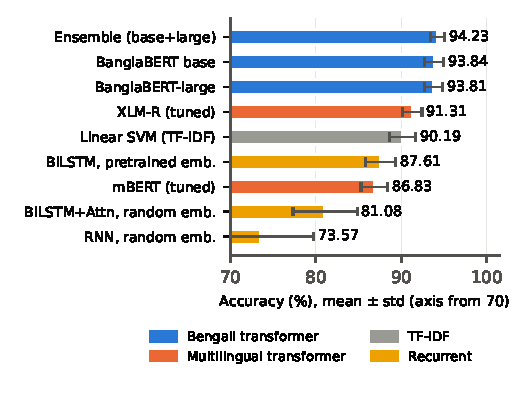
\includegraphics[width=\columnwidth]{fig2_bbr_bars.pdf}
\caption{Accuracy on BBR-2009 (three seeds $\times$ five folds; recurrent models five seeds). Bars show the mean and whiskers one standard deviation.}
\label{fig:bars}
\end{figure}

\subsection{Choosing among pretrained models}
Bigger is not better here. BanglaBERT-large (\pmstd{93.8}{1.0}\%) cannot be told apart from the base model (Wilcoxon $p=0.89$), and the base+large ensemble (\pmstd{94.2}{0.8}\%) is not significantly better either ($p=0.16$; McNemar's test finds a difference in only one of the three seeds). What does matter is pretraining on Bengali text: XLM-R reaches \pmstd{91.3}{1.1}\% and multilingual BERT \pmstd{86.8}{1.5}\%, in that order in every seed, and tuning moved them by at most 0.3 points. McNemar's test confirms that the ensemble beats the best TF-IDF model in every seed ($p<10^{-8}$). Calibration is reasonable (ECE 0.047, 0.057 and 0.041 for the base, large and ensemble models).

Table~\ref{tab:abl} shows that the result is not fragile: dropping class weights or raising the learning rate changes nothing, and shorter inputs or fewer epochs cost 0.6 to 0.7 points, within one standard deviation.

\begin{table}[t]
\centering
\caption{BanglaBERT ablation on BBR-2009 (3 seeds $\times$ 5 folds).}
\label{tab:abl}
\small
\renewcommand{\arraystretch}{1.18}
\begin{tabular}{@{}lcc@{}}
\toprule
Variant & Accuracy (\%) & $\Delta$ vs.\ default \\
\midrule
Default (lr $3{\times}10^{-5}$, 4 epochs) & \pmstd{93.84}{1.10} & -- \\
Learning rate $5{\times}10^{-5}$ & \pmstd{93.86}{1.31} & $+0.02$ \\
No class weights & \pmstd{93.83}{1.27} & $-0.01$ \\
Maximum length 64 & \pmstd{93.26}{1.42} & $-0.58$ \\
Two epochs & \pmstd{93.13}{1.21} & $-0.71$ \\
\bottomrule
\end{tabular}
\end{table}

\subsection{Other datasets and published results}
Fig.~\ref{fig:datasets}(a) and Table~\ref{tab:pub} put our numbers beside published ones. On the Mendeley corpus BanglaBERT reaches \pmstd{96.7}{1.2}\%, but Multinomial Naive Bayes already reaches \pmstd{94.2}{1.7}\% under our protocol. The 84\% reported earlier \cite{hossain2020} comes from the authors' own 2,000-review corpus, of which only 1,443 reviews are public, so that comparison is indicative at best. On Rokomari, BanglaBERT reaches \pmstd{90.6}{0.7}\% accuracy in cross-validation. The authors of \cite{sarker2022} report 88.95\% weighted F1 on a split we cannot reproduce, because their shuffle is unseeded. Following their protocol (positive and negative reviews of at most 300 words, stratified 80/10/10) with three random shuffles, BanglaBERT obtains $89.97\pm0.66$\% weighted F1. That is a point higher, but with a different split and about 500 test reviews it lies well within the shuffle-to-shuffle variation, so we do not count it as an improvement.

On the official BanglaBook split (Fig.~\ref{fig:datasets}(b)) we fall short. Our first runs reached 0.892 and 0.919 weighted F1, and one later run collapsed to the majority class (0.846); we adjusted these runs after seeing test scores, so they are shown only for transparency. We then fixed the protocol and chose everything on the validation set. Six runs (five BanglaBERT-large runs with different seeds, learning rates and class weights, and one BanglaBERT base run) each scored between 0.923 and 0.926 on the test set. Selecting the ensemble members and class offsets on the validation set picked three of the large runs, and their average scored \textbf{0.927} (accuracy 93.6\%, macro-F1 0.681). That is 0.6 points below the 0.933 reported in \cite{kabir2023}, and we do not claim to match it. Per-class F1 is 0.72, 0.36 and 0.97 (negative, neutral, positive) against 0.72, 0.40 and 0.97 in \cite{kabir2023}, so the gap sits in the neutral class.

\begin{figure*}[!t]
\centering
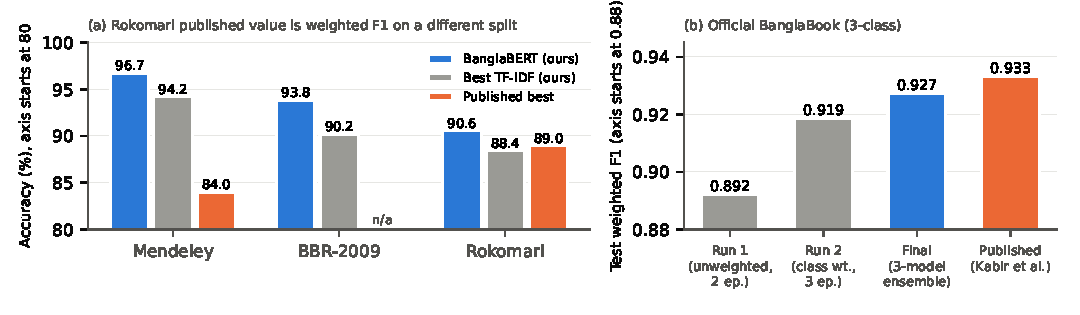
\includegraphics[width=\textwidth]{fig3_datasets.pdf}
\caption{(a) Our results against the best TF-IDF baseline and published results (the Rokomari published value is weighted F1 on a different split). (b) Official BanglaBook benchmark: weighted F1 of earlier runs, our final validation-selected ensemble and the published value.}
\label{fig:datasets}
\end{figure*}

\begin{table*}[!t]
\centering
\caption{Published results against ours. ``Comparable'' says whether the two numbers come from the same data and split.}
\label{tab:pub}
\small
\renewcommand{\arraystretch}{1.15}
\begin{tabular}{@{}lp{3.6cm}p{4.3cm}p{4.9cm}@{}}
\toprule
Dataset (metric) & Published & Ours & Comparable? \\
\midrule
Mendeley (acc.) & 84.0\% (Naive Bayes \cite{hossain2020}, authors' 2,000-review corpus) & \textbf{96.7\%} BanglaBERT; 94.2\% Naive Bayes & Indicative only: their corpus has 2,000 reviews, only 1,443 are public; Naive Bayes reaches 94.2\% on the public part \\
Rokomari (wF1) & 88.95\% (XLM-R \cite{sarker2022}) & \textbf{89.97 $\pm$ 0.66\%} BanglaBERT (their protocol, 3 shuffles) & No: their split cannot be reproduced; difference is within noise \\
BanglaBook (wF1) & 0.933 (BanglaBERT-large \cite{kabir2023}) & 0.927 (validation-selected ensemble) & Yes, official split. We are 0.6 points \textbf{below} \\
\bottomrule
\end{tabular}
\end{table*}

\subsection{What the model looks at}
We computed SHAP values for all 402 held-out reviews of an 80/20 split. Fig.~\ref{fig:shap} shows the most influential tokens: words meaning \emph{bad}, \emph{annoying} and \emph{worthless} push toward negative, and \emph{best}, \emph{excellent} and \emph{great} toward positive. A few function words and word pieces also show up, which hints at some dataset-specific cues.

An explanation can look convincing and still be unfaithful, so we tested it. We deleted the $k$ highest-SHAP tokens of each review and compared the drop in the predicted-class probability with deleting $k$ random tokens (Fig.~\ref{fig:noise}(a)). The SHAP-selected tokens are three to five times more influential ($k=1,3,5$: 0.120, 0.324, 0.444 against 0.024, 0.095, 0.150). Errors are not driven by negation words (4.7\% with one, 5.9\% without) or by length (4.2 to 7.0\% across quartiles); they follow the source instead, with an error rate of 12.1\% for BanglaBook reviews and 2.8\% for Mendeley reviews.

\begin{figure}[t]
\centering
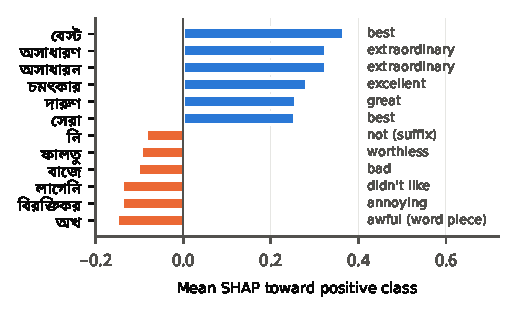
\includegraphics[width=0.88\columnwidth]{fig5_shap.pdf}
\caption{Tokens with the largest mean SHAP contribution to the positive class (402 held-out reviews; orange pushes toward negative, blue toward positive). English glosses are added for readers who do not read Bengali.}
\label{fig:shap}
\end{figure}

\begin{figure*}[!t]
\centering
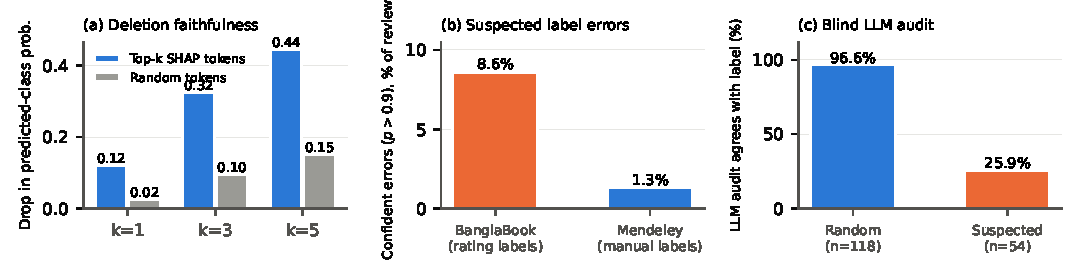
\includegraphics[width=\textwidth]{fig4_explain_noise.pdf}
\caption{(a) Deleting top-$k$ SHAP tokens lowers the predicted-class probability much more than deleting random tokens. (b) Share of reviews on which the ensemble is confidently wrong ($p>0.9$), by source. (c) Agreement between a blind LLM annotator and the dataset label for random and suspected reviews.}
\label{fig:noise}
\end{figure*}

\subsection{Label noise and transfer}
The source effect raises a question: are some of these ``errors'' actually wrong labels? Pooling out-of-fold predictions over three seeds and both model sizes, the ensemble misclassifies 111 of 2,009 reviews, and 69 of those errors (62\%) were made with a probability above 0.9. A model that sure and still at odds with the label deserves a second look. These cases cluster in the rating-derived source: 51 of 595 BanglaBook reviews (8.6\%) against 18 of 1,414 Mendeley reviews (1.3\%) (Fig.~\ref{fig:noise}(b)).

To look closer, we shuffled the 69 suspected reviews with 131 random ones, removed every label and asked a single large language model to label them from the text alone. It judged 28 reviews unclear, and we dropped them. On the random reviews it agreed with the dataset label 96.6\% of the time (Cohen's $\kappa=0.93$), so it is not just contradicting the data. On the suspected reviews agreement fell to 25.9\% ($\kappa=0.00$), and 39 of the 43 reviews labeled negative were judged positive (Fig.~\ref{fig:noise}(c)). Table~\ref{tab:examples} shows what these cases look like: three of the five are clearly positive reviews carrying a negative label, which is what one expects when a one- or two-star rating becomes a label, and the other two are genuine model mistakes. The list is therefore a mix and not a clean set of label errors. Since the annotator is a single LLM and not a human study, we treat this as a strong hint, not as ground truth.

Cross-source transfer tells a similar story (Fig.~\ref{fig:transfer}). A model trained on Mendeley reaches 84.5\% on Rokomari, and one trained on Rokomari reaches 91.2\% on Mendeley, but both transfer poorly to the BanglaBook reviews (77.0\% and 82.4\% accuracy; macro-F1 58.3 and 63.8).

\begin{table*}[!t]
\centering
\caption{Examples of confident disagreements (English translations of the Bengali reviews). The first three look like wrong labels, the last two like model mistakes.}
\label{tab:examples}
\small
\renewcommand{\arraystretch}{1.15}
\begin{tabular}{@{}p{7.2cm}clcp{3.1cm}@{}}
\toprule
Review (translated) & Dataset label & Model $P$(pos.) & Source & Likely cause \\
\midrule
``Truly a very good book'' (two heart-eyes emoji) & neg. & 0.99 & BanglaBook & label (rating) \\
``I liked it a lot, thank you to the author.'' & neg. & 0.99 & BanglaBook & label (rating) \\
``An extraordinary book; without it I would not have learned about many forbidden matters.'' & neg. & 0.99 & BanglaBook & label (rating) \\
``There is no equal to this book.'' & pos. & 0.002 & Mendeley & model: misread idiom with a negation word \\
``A good book, but I saw quite a few printing mistakes, and an alphabetical index would have helped.'' & pos. & 0.004 & Mendeley & model: mixed review \\
\bottomrule
\end{tabular}
\end{table*}

\begin{figure}[t]
\centering
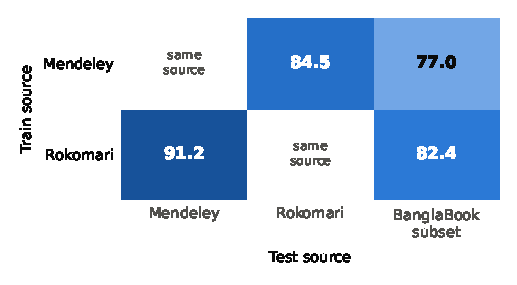
\includegraphics[width=\columnwidth]{fig7_transfer.pdf}
\caption{Cross-source transfer of BanglaBERT (accuracy \%, single seed). Models trained on a manually labeled or Rokomari source transfer poorly to the rating-labeled BanglaBook reviews.}
\label{fig:transfer}
\end{figure}

\section{Discussion and Limitations}
Three things stand out. First, a single split can mislead: one model scores anywhere from 73\% to 86\% depending on the fold. Second, what separates the models is pretraining on Bengali text, first of the embeddings and then of the whole encoder, and not recurrence, attention or model size; a TF-IDF baseline is also often stronger than the one used for comparison in earlier papers. Third, some of what looks like model error is label error, especially in rating-derived data, so accuracy on such corpora understates what a model can do.

The study has limits. BBR-2009 is small, rebuilt from two sources of different origin, and partly confounded by source, and rating-derived labels are noisy. The audit used one LLM annotator, which may share blind spots with BanglaBERT, so the suspected errors are not confirmed; independent human annotation is the obvious next step. The Rokomari experiments used a different split from the published one, and on the official BanglaBook benchmark we remain 0.6 points behind. The recurrent and classical baselines were not tuned (pretrained embeddings narrow the gap to BanglaBERT but do not close it), our Wilcoxon tests treat cross-validation runs as independent and are therefore somewhat optimistic, and XLM-R and mBERT were tuned over a small grid only. We also did not test large language models with few-shot prompting.

\section{Conclusion}
Under repeated cross-validation, recurrent models trained from scratch reach about 81\% on Bengali book reviews, while fine-tuned BanglaBERT reaches 93.8\% on our corpus and 96.7\% on the Mendeley corpus. The explanations we checked are faithful, and many of the model's confident errors look like label errors. We hope the released splits and this frank comparison make future results easier to trust. Next we plan independent human re-annotation, few-shot large language models, and larger, manually verified Bengali review corpora.

\section*{Availability}
The BBR-2009 text, labels, source flags, fold assignments and datasheet will be released for non-commercial use (CC BY-NC-SA 4.0, inherited from BanglaBook), together with code and logs, at \url{https://github.com/NoorAbdullah02/bbr2009-bengali-book-review-sentiment}.

\section*{Acknowledgment}
We thank the creators of the Mendeley, BanglaBook and Rokomari review datasets for making their data available.

\bibliographystyle{IEEEtran}
\bibliography{refs}

\end{document}
